\def\year{2018}\relax
%File: formatting-instruction.tex
\documentclass[letterpaper]{article} %DO NOT CHANGE THIS
\usepackage{aaai}  %Required
\usepackage{times}  %Required
\usepackage{helvet}  %Required
\usepackage{courier}  %Required
\usepackage{url}  %Required
\usepackage{graphicx}  %Required
\usepackage{fullpage,enumitem,amsmath,amssymb,graphicx,listings, float,stmaryrd, textcomp, algorithm}
\usepackage[noend]{algpseudocode}
\frenchspacing  %Required
\setlength{\pdfpagewidth}{8.5in}  %Required
\setlength{\pdfpageheight}{11in}  %Required
%PDF Info Is Required:
  \pdfinfo{
/Title (CS 257 Final Project)
/Author (Makai Mann)}
\setcounter{secnumdepth}{0}  
 \begin{document}
% The file aaai.sty is the style file for AAAI Press 
% proceedings, working notes, and technical reports.
%
\title{CS 257 Final Project \\ Towards Learning in SAT-based Bounded Model Checking}
\author{Makai Mann \\
21 March 2018
}
\maketitle
\begin{abstract}
SAT-based bounded model checking (BMC) is a state of the art formal verification approach for bug-finding. In a BMC run, a SAT solver is queried multiple times as the circuit is \textit{unrolled} over time. This sequence of queries is unsatisfiable until a potentially satisfiable call, when a counterexample is found. This paper explores machine learning techniques to learn from the unsat proofs of previous unrolls and applies the learned model to guide the SAT solver in subsequent unrolls. This project is focused on prototyping and thus makes use of existing, open source tools whenever possible.
\end{abstract}

\section{Introduction}
\noindent As digital circuits become increasingly complex, more and more of the time to produce a new design is spent in verification and validation. Formal approaches such as hardware model checking have arised as a popular complement to simulation based testing for catching bugs (and even proving correctness) earlier in the design process. Formal tools can reason over the design symbolically, which circumvents the primary challenge of simulation-based testing: the exponentially growing input space. Despite the relative success and broad adoption of these techniques in industry, formal tools still face scaling issues on larger designs. To prevent security flaws such as Meltdown and Spectre, and to save chip design companies huge sums of money spent on preventing and mitigating bugs, it is vital to address the scaling concerns of formal tools.

One of the most popular techniques is bounded model checking, which produces a bounded proof that a property holds. Typically, the bounded model checker iteratively increases the bound until it times out or finds a counter example trace. Intuitively, it seems that this sequence of calls to a formal solver might be related because each query is the same circuit unrolled over increasing time-steps. Therefore, it seems plausible that machine learning techniques could learn to guide the formal tool based on previous queries.

\section{Background}
This paper assumes basic knowledge of propositional logic. Below, I will begin by setting up the hardware model checking problem, describe the details of SAT-based bounded model checking, and finish by reviewing SAT solver's interpretation as resolution theorem provers. All of these topics are important for understanding the learning portion of this report.

\subsection{Hardware Model Checking}
Hardware model checking regards a digital circuit written in a representation language such as Verilog or VHDL as a symbolic finite state machine. Given the circuit description, some environmental assumptions and a property in a temporal logic, the model checking problems determines if the property holds. For the context of this report, I restrict focus to safety properties -- that a bad state is not reachable. It has been shown that other types of properties, such as liveness (something good eventually happens) can be reduced to safety checking \cite{biere}. Figure \ref{hwmc} shows the typical hardware model checking structure.

In the early days of model checking, explicit state techniques such as tableau methods were the focus. Since then, symbolic model checking has become the standard approach. Symbolic model checkers reason over sets of states as opposed to concrete states. SAT-based techniques encode the symbolic model checking problem into one or more SAT queries. This family of approaches includes algorithms which can definitely prove properties such as k-induction and property directed reachability, as well as bounded techniques such as bounded model checking, which can only find bugs. For many classes of circuits, bounded model checking is the fastest approach for finding obscure bugs.

\begin{figure}[H]
\begin{center}
  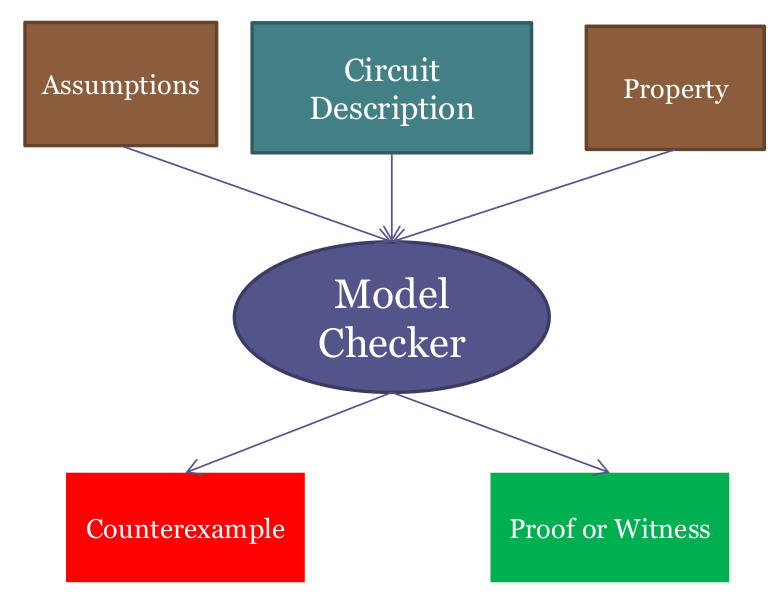
\includegraphics[scale=0.2]{hwmc.png}
  \caption{Hardware Model Checking setup}
  \label{hwmc}
\end{center}
\end{figure}

\subsection{SAT-based Bounded Model Checking}
In SAT-based bounded model checking, each bit of the circuit is given a SAT literal and the combinational logic is represented with SAT formulas. To capture the behaviour of sequential elements, the literals are duplicated for each clock cycle and constrained with a transition relation that models the circuit behaviour.

Formally, $M := <V, I, T>_k$ describes the SAT encoding at bound $k$. Where, 
\begin{equation*}
\begin{split}
V &= \{B_0^{(0)} \dots B_{n}^{(0)} \dots B_{n}^{(k)}\} \text{, the SAT variables} \\
I &= \text{The formula describing the initial state} \\
T &= \text{The formula capturing the relation} \\
&  \ \  \ \  \ \  \text{between current and next state elements}
\end{split}
\end{equation*}

Then by checking if $M \models P$ for some property formula $P$, we are checking if there is any trace violating the property in $k$ time-steps.

\subsubsection{2-bit Counter Example}

A simple 2-bit counter with the clock abstracted (next states are the state after a full clock cycle) can be described at $k=1$ as follows:

\begin{equation*}
\begin{split}
V &= \{C_1^0, C_0^0, C_1^1, C_0^1\} \\
I &= \neg C_0^1 \wedge \neg C_0^0 \\
T &= C_0^1 \oplus C_0^0 \wedge \\
& \neg (C_1^1 \oplus (C_1^0 \oplus C_0^0))
\end{split}
\end{equation*}
This starts the counter at $00$ in the initial state and the transition relation evaluates to true exactly when the next state is the current state incremented by one. As $k$ increases, the transition relation is repeated for each pair of related states. This large propositional formula is then converted to conjunctive normal form (CNF) and passed to a SAT solver along with the negated property. A \textit{clause} refers to a disjunction of literals in CNF. A satisfiable result gives a model assignment which is a counter example trace. An unsatisfiable result means the property holds up until bound $k$.  

Thus, in a typical bounded model checking run, there is a sequence of $k-1$ unsatisfiable queries to the SAT solver, after which there is either a timeout or one satisfiable query, in which case a bug is identified and the SAT model gives a counterexample trace. Thus, to speed up bounded model checking it behooves us to focus on unsatisfiable queries, because they make up the bulk of the effort. Furthermore, unsatisfiable queries are able to produce a lot of potentially useful data in the form of an unsat proof.

\subsection{SAT Solvers as Resolution Theorem Provers}

A common form for a proof of unsatisfiability is a resolution refutation proof. This proof is represented as a DAG where each node is a clause. Each node is either a leaf, meaning it was part of the original clauses given in the SAT query, or has two parents. The parents are each clauses that have been resolved on a literal to produce the child clause. A resolution DAG always ends in the empty clause which demonstrates that the original queries were unsatisfiable. While resolution is a sound and complete technique for proving unsatisfiability, there are exponentially many ways of producing clause resolutions and in practice this approach does not perform well. Rather, the most common modern approach is to use a conflict-driven clause learning (CDCL) SAT solver.

Although CDCL SAT solvers do not employ clause resolution very often, they can still produce resolution refutation proofs. In fact, it has been shown that CDCL solvers p-simulate general resolution for propositional logic \cite{cdclres}.

In the process of solving a SAT problem, CDCL solvers find \textit{conflicts}: a known clause from the database which is falsified by the current assignment of literals. Once a conflict has been found, it can be modified by resolving on literals forced by unit propagation in the current assignment trail. This produces a learned clause which is then added to the database, preventing the SAT solver from exploring this part of the space again. For more detailed coverage of this topic, see \cite{satres}.

\subsubsection{Antecedent Graphs}

Resolution proofs can grow exponentially large, thus the SAT community developed a trace format which represents a resolution proof in a more compact format. The trace format represents the proof as an antecedent graph where there are edges between clauses and the learned clauses they produce. Unlike a resolution proof, each node in the graph can have more than two parents. The parents are not required to be in any particular order, but by applying clause resolution between the parents, it is possible to derive the child.

The learning phase of this project will take a resolution proof or antecedent graph as inputs and attempt to learn some underlying structure of the circuit.

\subsection{Supervised Learning}
Supervised learning aims to construct a classification or regression function based on a set of data points and their associated labels. The reader is assumed to be familiar with basic supervised learning techniques. Thus, the learning algorithms are omitted from the background section. The curious reader can refer to \cite{Murphy} for a complete introduction.

\section{Learning from Previous Queries}

Given an unsat proof from the $(k-1)th$ bounded model checking call, a machine learning algorithm can learn a scoring function which can identify useful clauses at bound $k$. Then, a procedure will generate many resolvents and the scoring function can be used to decide which resolvents to keep. Furthermore, the function can actually be used to direct the clause resolution online towards more useful resolvents.

The discussion below starts with a description of the normal form transformation used for all SAT literals, continues with various feature selection techniques and concludes with the method for assigning labels. The majority of this project consisted of defining and producing the right data, and only then trying multiple algorithms for model learning.

\subsection{Normal Form}
The goal is to learn to score useful clauses, thus the input to the scoring function will be a clause in some processed form. The first fundamental transformation I applied was mapping all literals in a clause to an equivalence class.

In the BMC query, there is a new literal for every bit in the circuit for every time step. Thus, rather than including all literals, I chose a representative for each physical wire and mapped all literals to that one literal. For example, the following expressions (given in SMT-LIB notation) would each receive a literal in the SAT transformation, and would be mapped to a normal form:

\begin{equation*}
\begin{split}
&\text{(= wrPtr@4 (+ wrPtr@3 \#b0001))} \\
&\to \text{(= wrPtr@(k+1) (+ wrPtr@k \#b0001))} \\
&\text{(= wrPtr@3 (+ wrPtr@2 \#b0001))}\\
&\to \text{(= wrPtr@(k+1) (+ wrPtr@k \#b0001))}
\end{split}
\end{equation*}

\noindent where "@" is a naming scheme which annotates the signal name with the time-step.

In practice, the representative literal is chosen arbitrarily as the first instance of a signal. 

The normal form is important so that the machine learning algorithm does not have to recover temporal relations between these literals that is already known. This transformation is inspired by other symbolic model checking techniques such as Binary Decision Diagram techniques and Property Directed Reachability (PDR). Both of these approaches are based on fixpoint computations which iteratively calculate all reachable states over the transition relation without unrolling the circuit. Instead they only look at the current and next state abstractly. PDR in particular is similar to this normal form transformation in that it extends the trace length, but adds each new reachable state to the abstract representation.

The normal form of a clause is simply the clause produced by mapping all of its literals to their normal form, and sorting them in ascending order. Sorting the literals in the clause ensures that a given clause has only one representation. This is important so that the learning algorithm can easily identify each clause without identifying that order of literals in the clause does not matter.

\subsection{Features}

Now that we have a normal form for each clause, they have to be represented as a vector of features for the learning algorithm. There are multiple representation approaches, two of which will be covered below.

\subsubsection{Sampled Literals}

A clause can have an unbounded number of literals, making it impossible to represent every possible clause as a vector. One approach is to simply sample $N$ of the literals and include them as an integer representation, where $- := \neg$. This is based on the common input format DIMACs for SAT queries. Furthermore, in this approach, I also append the size of the original clause. Thus, the learning algorithm can infer a relation between clause size (since if $size > N$, only a subset of the literals are being used) and the score, if it exists.

\subsubsection{One-Hot Literals}

Another possible representation of a clause is a "one-hot literal". In this context of this project, the number of possible literals, $M$, is known after computing the normal form. Thus we can form a vector $v$ of length $M$ for each clause. Again, we consider literals as integers and if the literal, $l$, appears in the clause, then $v_l \gets 1$. If the negated literal, $-l$ appears in the clause, then $v_{-l} \gets -1$. This one-hot approach has been shown to be successful in other classification problems.

\subsubsection{Bounds}

Finally, I also include the minimum and maximum bounds represented in each clause as the last two elements of the feature vector. Although the normal form is important for ensuring that the learning algorithm can relate the signals over time, there could be interesting temporal information. Thus, including the bounds might help for learning temporal relations.

Using the example from earlier, the minimum and maximum bounds of a literal are:

\begin{equation*}
\begin{split}
&\text{(= wrPtr@4 (+ wrPtr@3 \#b0001))} \\
&min\_bnd := 3 \\
&max\_bnd := 4
\end{split}
\end{equation*}

The minimum bound of a clause is defined as the minimum over all the minimum bounds of literals in the clause, and similarly for the maximum bound.

\subsection{Labels}
The simplifying assumption for labeling in this project is that clauses appearing closer to the end of a resolution proof are more useful. It is unclear if this is true in general. However, this seems reasonable because if the parents of the empty clause in a resolution proof were added to the clause database before solving, then the problem becomes trivial. 
\subsubsection{Resolution Proof}
A resolution proof can be represented as a DAG. Any clause from the original query that does not appear in the resolution DAG is given a score of $0$. Based on the simplifying assumption above, I score each clause by traversing the graph in a breadth-first manner starting at the empty clause. The parents of the empty clause get the highest scores, and their parents get their score minus one, and so on. In practice, the depth of the resolution DAG might not be known before traversing, so the scores are adjusted to be positive after the traversal. The outline of the algorithm is in Algorithm \ref{scoring}.

\begin{algorithm}
\caption{Score Clauses}\label{scoring}
\begin{algorithmic}[1]
\Procedure{score}{$empty\_clause\_node$}
\State $node\_queue = parents(empty\_clause\_node)$
\State $score[empty\_clause\_node.clause] \gets 0$
\State $min\_score \gets \infty$
\For{$p$ in $node\_queue$}
\State $node\_queue.add(parents(p))$
\State $score[p.clause] \gets $
\State \ \ \ \ \ \ \ \ \ $score[p.clause.child] - 1$
\If {$score[p.clause] < min\_score$}
\State $min\_score \gets score[p.clause]$
\EndIf
\EndFor
\For{$c, s$ in $score$}
\State $score[c] \gets score[c] - min\_score$
\EndFor
\State return $score$
\EndProcedure
\end{algorithmic}
\end{algorithm} 

Once all the clauses are scored, I have another procedure which groups the scores into $N$ categories. So if $N=8$, the maximum score is divided by $8$ and every score is then adjusted to be in $\{0, \dots, 7\}$. This allowed me to try various different magnitudes for the scores.

\subsubsection{Unsat Trace}
In practice, I found that resolution proofs quickly became prohibitively large. For small unrolls the full resolution proof was nice for providing enough data to a learning algorithm, but in later bounds it was simply too large. In that case, the scoring procedure can be applied in exactly the same way to an antecedent graph produced by a SAT solver. The only difference here is that a node may have more than two parents.
\subsubsection{Classification vs. Regression}
In this case, the labels are always integers. From here, I could treat the learning as either a classification problem, where the output is always an integer (more broadly, a category) or a regression problem which can approximate with floating point numbers. My intuition is that a regression approach would be more effective and that I can use those scores only relative to the scores of other clauses. This could also help to guide the clause resolution step towards resolvents with higher scores. In practice, I also found that regression algorithms tended to be more accurate. This will be covered more in the results section.
\section{Implementation}
My implementation is primarily written in Python, but makes use of several C++ tools and libraries. The code is available on \url{https://github.com/makaimann/cs257proj}. Because of Github restrictions on file sizes, I did not include the compiled binary of CVC4 with debug symbols.
\subsection{Toolflow}
This project made use of several open source tools which allowed for easy prototyping. I provided some "glue" code, primarily in Python for connecting the various tools. The first goal was to take a design written in Verilog and produce a SAT BMC query, while also keeping track of the mapping between signals and SAT variables. The mapping is crucial for establishing the normal form discussed above. Figure \ref{toolflow} depicts the toolflow used in this project. Brown ovals represent representation formats and blue rectangles are tools.

\begin{figure}
\begin{center}
  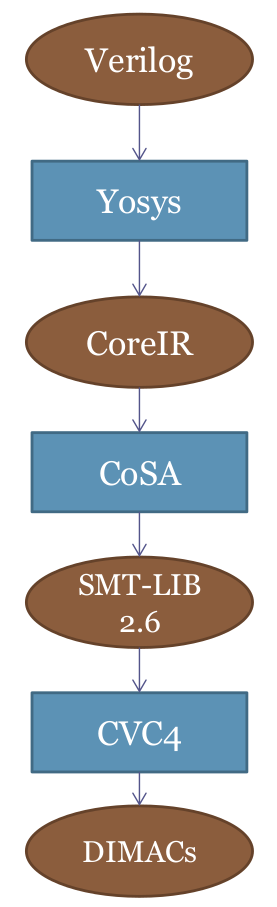
\includegraphics[scale=0.2]{flow.png}
  \caption{Tool Flow}
  \label{toolflow}
\end{center}
\end{figure}

\subsubsection{Formats}

\begin{enumerate}
\item Verilog: A popular hardware description language
\item CoreIR: An intermediate representation for hardware designs developed here at Stanford
\item SMT-LIB 2.6: The format for queries to a Satisfiability Modulo Theory (SMT) solver
\item DIMACs: The format for queries to a SAT solver
\end{enumerate}

\subsubsection{Tools}

\begin{enumerate}
\item Yosys: An open source Verilog synthesis tool. The CoreIR developers have written a pass over Yosys's internal representation which I used to output CoreIR
\begin{enumerate}
\item \url{https://github.com/YosysHQ/yosys}
\end{enumerate}
\item CoSA: The CoreIR Symbolic Analyzer is a model checking framework written in Python out of Dr. Clark Barrett's group for setting up various model checking queries of CoreIR designs.
\begin{enumerate}
\item \url{https://github.com/cristian-mattarei/CoSA}
\end{enumerate}
\item CVC4: A leading SMT solver with support for various theories including quantifier free bit-vectors, which is what I used in this project. CVC4 does not have native support for outputting a DIMACs file. However, there are various debug prints which output every DIMACs clause added and mappings between SMT-LIB formulae and SAT literals. I wrote a Python script which reads these debug prints, constructs the DIMACs file and saves the mapping for use in the normal form transformation.
\begin{enumerate}
\item \url{https://github.com/CVC4/CVC4}
\end{enumerate}
\end{enumerate}

\subsection{Data Collection}

With the toolflow described above, I can translate a Verilog circuit into a SAT BMC query and keep track of literals unrolled over time. The next step is to generate input data for a learning algorithm.

In Python I wrote classes for clauses, literals and DAG nodes. The clauses support various useful methods regarding resolution and can be "registered" with their literals. When a clause is registered, each of it's literals gets a pointer to the clause. This is useful for identifying candidate clauses for resolution in an efficient manner. 

I used the SAT solver Picosat to produce an antecedent graph trace file. Then, I used a tool called tracecheck, which is distributed with the Booleforce SAT solver to reconstruct a resolution proof from the trace file. 

I also provided functions for parsing these text files into my Python representation of a resolution DAG (or antecedent graph). Then, each of the clauses are scored according to the procedure in Agorithm \ref{scoring}. Finally, a python function converts these clauses into either the sampled literal feature form or the one-hot literal feature form. At this point, I have a collection of feature vectors with their associated labels.

\subsection{Learning Framework}

For the learning portion of this project, I used the popular machine learning library scikit-learn, \url{https://github.com/scikit-learn/scikit-learn}.  This tool has support for all of the main machine learning algorithms as well as convenience functions for manipulating data, including generating validation sets. For each data set, I used scikit-learn to produce a $10\%$ validation set for performance evaluation.

\subsubsection{Evaluation Metrics}

There are two main evaluation metrics used in this project. For regression algorithms, I used percent mean absolute error (MAE). This is the MAE divided by the maximum score (to normalize the magnitude of the MAE). For classification algorithms, I simply used the percentage of misclassifications.

\begin{equation*}
\begin{split}
\% MAE &= \frac{\Sigma_{y_{test}} abs(y_{test} - y_{predict})}{max\_score} \\
\% misclassified &= \frac{\Sigma_{y_{test}} \textbf{1}[y_{test} != y_{predict}]}{\text{Number of test points}}
\end{split}
\end{equation*}

\subsubsection{Machine Learning Algorithms}

I tried the following algorithms in this project:

\begin{enumerate}
\item Support Vector Machine Classifier
\item Support Vector Machine Regressor
\item K-Nearest Neighbor Classifier
\item K-Nearest Neighbor Regressor
\item Multilayer Perceptron Classifier
\item Multilayer Perceptron Regressor
\item Gaussian Process: Never completed due to memory issues
\item Logistic Regression
\item AdaBoost Classifier
\item RandomForest Classifier
\end{enumerate}

\subsection{Applying the Model}

Once there's a model which can be used to score clauses, I run Algorithm \ref{genclauses} (again implemented in Python) parameterized by $B$, the number of burn iterations, $N$, the desired number of clauses, and $p$ the percent of generated clauses to add. To help with this algorithm, I use a max-heap which keeps clauses sorted by their score. As can bee seen in line 13, this algorithm actually guides the clause resolution towards resolvents with higher scores by iterating over the top clauses and only keeping clauses with scores higher than their parents.

\begin{algorithm}
\caption{Generate Clauses}\label{genclauses}
\begin{algorithmic}[1]
\Procedure{genclauses}{$model, clauses, B, N, p$}
\State $gen\_clauses := max-heap$
\For{$i = 0$; $i < B$; $i++$}
\State Generate a random resolvent, $r$
\State $model.score(r)$
\State $gen\_clauses.push(r)$
\EndFor
\While{Number of new clauses $\leq N$}
\For{$c$ in $gen\_clauses.top(30)$}
\For{$c2$ in $c.resolvable\_clauses()$}
\State $cr \gets resolve(c, c2)$
\State $max\_score =$
\State \ \ \ \ \ \ \ $max(model.score(c),$ \State \ \ \ \ \ \ \ \ \ \ \ \ \ \ \ \ $model.score(c2))$
\If{$model.score(cr) \geq max\_score$}
\State $gen\_clauses.push(cr)$
\EndIf
\EndFor
\EndFor
\EndWhile
\State return top $p\%$ of $gen\_clauses$
\EndProcedure
\end{algorithmic}
\end{algorithm} 

\section{Experimental Setup}

To evaluate the efficacy of scoring resolvents for speeding up BMC, I train a network on the unsat proof of a circuit unrolled to bound $k$. Then, read in the clauses for bound $k+1$, generate a bunch of resolvents guided by learned model. I add the highest-scored clauses back to the DIMACs file for bound $k+1$ (which is sound because clause resolution is always sound) and compare the solve times between the modified and original DIMACs.

\subsection{Case Study Benchmark}

For a case study, I used a bounded data integrity proof for a FIFO implementation with circular pointers. A packet is nondeterministically (i.e. the solver can choose which packet to track) chosen, the value saved, and the location tracked with a counter. When that packet is supposed to be exiting, it is expected to be equivalent to the saved value. Figure \ref{mp} demonstrates the relationship between the packet counter and the pointers.

This fifo has data width 8 and depth 8. Although this problem seems simple, it is actually relatively challenging in the BMC context for most SAT solvers. This is related to the many possible combinations of state values, and path variables (when to push or pop).

\begin{figure}
\begin{center}
  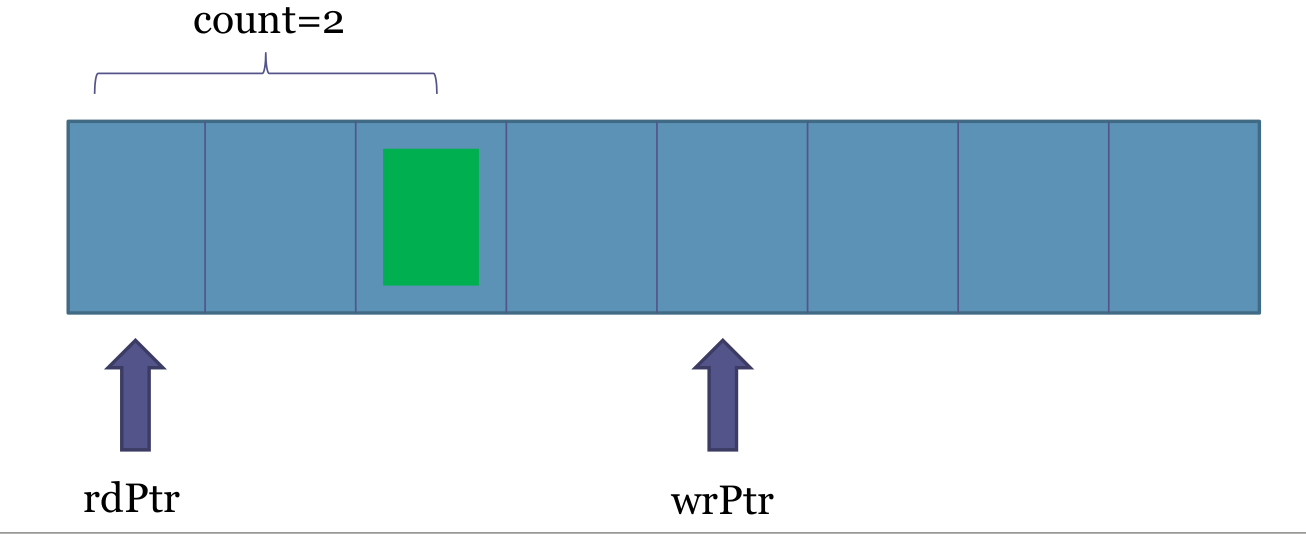
\includegraphics[scale=0.15]{magicpacket.png}
  \caption{Relationship between packet tracking counter and read pointer}
  \label{mp}
\end{center}
\end{figure}

\section{Results}

All experiments were run on Ubuntu 16.04 running on an Intel(R) Core(TM) i7-6700HQ CPU @ 2.60GHz.

\subsection{Machine Learning Accuracy}

Tables \ref{acc-class} and \ref{acc-reg} show accuracy results of the various machine learning algorithms on a $10\%$ validation set removed from the original training data for the data integrity example unrolled to bound 10.  I normalized the scores to be integers from 0 to 7.

%\begin{table}[h!]
\begin{table}[h!]
\centering
\begin{tabular}{ c | c | c }
Algorithm & Feature encoding & \% Misclassified \\
\hline \\
AdaBoost & Sampled & 62.842\% \\
RandomForest & Sampled & 11.441\% \\
Support Vector Machine & Sampled & 10.260\% \\
Multilayer Perceptron & Sampled & 17.852\% \\
KNN & Sampled & 10.280\% \\ 
AdaBoost & One-hot literal & 16.53\%\\
RandomForest & One-hot literal & 12.654\% \\
Support Vector Machine & One-hot literal & 15.357\% \\
Multilayer Perceptron & One-hot literal & 23.497\% \\
KNN & One-hot literal & 13.8987\% 
\end{tabular}
\caption{Classifiers Accuracy Results}
\label{acc-class}
\end{table}

\begin{table}[h!]
\centering
\begin{tabular}{ c | c | c }
Algorithm & Feature Encoding & \% MAE \\
\hline \\
Support Vector Machine & Sampled & 6.014\% \\
Multilayer Perceptron & Sampled & 23.45\% \\
KNN & Sampled & 5.044\% \\ 
Support Vector Machine & One-hot literal & 15.357\% \\
Multilayer Perceptron & One-hot literal & 23.497\% \\
KNN & One-hot literal & 26.528\% 
\end{tabular}
\caption{Regressors Accuracy Results}
\label{acc-reg}
\end{table}

\subsection{BMC Performance on Case Study}

The runtimes in the results do not include the training time for the machine learning model. In my current implementation, the training time is slow because Python is slow manipulating the large number of clauses. A performant implementation in a faster language such as C++ would solve this issue. If this technique were actually applied, I would expect the learning to be done in a separate thread and we could always use additional GPUs to speed up the training time. Furthermore, in a real implementation, the training time should scale better than the SAT solving time as the bound increases.

To compare performance, I add high-scoring generated clauses to the DIMACs file of the current bound. This process starts with a "burn" phase in which $B$ literals are sampled and all possible resolvents (in one step) involving each literal are generated. Those resolvents are scored and added to a max-heap. I used $B=100$. Then, I repeatedly iterate over the $30$ highest scoring clauses. At each iteration, I add every possible resolvent producible by that clause (with the current clause database). The procedure terminates when the number of added (post-burn) clauses is greater than a user defined-value $N$. For example, at bound 21 I used $N=20,000$. 

I also found it to be helpful to narrow the search towards the end. When it's close (about 90\% of the way) to $N$ clauses, start iterating only over the top $5$ clauses to hopefully discover "deep" resolvents. At the end, the top $10\%$ of the scored, generated clauses are appended to the DIMACs file. Table \ref{benchmark} shows the performance at a few increasing bounds. For each one, the model was trained on the previous bound and used to add resolvents of clauses involving literals from $bound-1$ to $bound+1$. In other words, only resolvents at the end of the unrolling were added.

For these results, I used the machine learning model with the best accuracy, which was the KNN regressor.

\begin{table}[h!]
\centering
\begin{tabular}{ c | c | c }
Bound & Modified & Time (sec) \\
\hline \\
4 & No & \\
4 & Yes & \\
11 & No & \\
11 & Yes & \\
21 & No & \\
21 & Yes & \\
\end{tabular}
\caption{Performance on Case Study}
\label{benchmark}
\end{table}

\section{Analysis}

Although it took some tuning, I was quite surprised at how accurate some of these machine learning models were even over this combinatorial feature space. That being said, the fact that KNNs were the most performant approach is a little bit concerning. Because KNN is just a voting scheme based on caching all the data, this makes me wonder if machine learning is even needed at all. Maybe the performance improvement could be achieved simply by adding the equivalent clauses at the next bound (as long as that clause cannot be traced back to the property in the resolution proof, which would be unsound). This will take more investigation to be sure about.

Furthermore, it is worth noting that the added clauses are often very similar. For example, in the most effective case, the FIFO at bound 21, all 2000 added clauses had two literals, one of which was the same in all of them. Similar clauses receive similar scores, so it makes intuitive sense why this happens. But at this point, it is unclear if this is desirable.

Despite my reservations, it was encouraging that the performance improvements seemed to increase as the bound increased. This is in line with the intuition that a machine learning model is more useful as it has more data and that the deeper bounds might benefit more from pruning the search space. I hope to continue trying additional bounds and models, but the Python implementation starts to get prohibitively slow as the number of clauses increases.

\section{Future Work}

I would like to investigate my concerns about the KNN performance. This should be easy to evaluate. There is a deterministic algorithm for lifting clauses over time steps, and I can compare the performance improvement of that against the scoring function approach.

Additionally, this approach has used naive bounded model checking which creates a new SAT solver instance for each bound. The natural next step would be to score and generate clauses online and use the SAT solver incrementally.

In general, I plan to evaluate this approach more. Based on my experience thus far, the performance is sensitive to the various parameters. I plan to spend some more time tuning these parameters and evaluating this technique at deeper bounds and on other examples. If this approach continues to be promising after these additional experiments, I will reimplement the learning and clause generation portion of the code base so that it is no longer the runtime bottleneck.

\section{Conclusion}

In conclusion, I have demonstrated promising results for incorporating learning into SAT-base bounded model checking. There is a lot of space for future work, and I believe after a few months of experimentation, I will know if this approach is practically applicable.

\section{Acknowledgements}

Thank you to Dr. Thomas Icard and Francesca Zaffora Blando for the great class and the opportunity to work on this project. Additionally, I want to thank my advisor Dr. Clark Barrett for his guidance and the initial idea to learn from unsat proofs in BMC. 

\bibliographystyle{aaai}
\bibliography{report}

\end{document}